% Bab 4: Point of Interest (POI) & Location-Trigger Design
\chapter{Point of Interest (POI) \& Location-Trigger Design}
\label{bab:point-of-interest-poi-location-trigger-design}
\section{POI Definition}

Dataset POI disimpan di \texttt{frontend/src/data/pois.json} dan dibundel di dalam APK. Dataset memuat 31 tenant di kawasan Sudirman Street Food (pusat kawasan $-6.92089$, $107.60057$; geofence kawasan radius 100 m). Semua POI memakai radius trigger 10 m (change log v1.1). Selain proximity event, setiap POI juga memicu dwell event (\(\ge\)3 menit di dalam radius) dan exit event (jarak \textgreater{} radius + 10 m), seperti dijelaskan pada F02. ID P02 dan P24 tidak dipakai.

\begin{landscapepage}
\begin{longtable}{|L{0.06}|L{0.17}|L{0.14}|L{0.14}|L{0.21}|L{0.11}|L{0.17}|}
\caption{POI Definition}\\
\hline
\cellcolor[HTML]{D9EAF7}\textbf{POI ID} & \cellcolor[HTML]{D9EAF7}\textbf{Nama POI} & \cellcolor[HTML]{D9EAF7}\textbf{Kategori} & \cellcolor[HTML]{D9EAF7}\textbf{Lokasi / Koordinat} & \cellcolor[HTML]{D9EAF7}\textbf{Content} & \cellcolor[HTML]{D9EAF7}\textbf{Trigger Rule} & \cellcolor[HTML]{D9EAF7}\textbf{System Response} \\ \hline
\endfirsthead
\hline
\cellcolor[HTML]{D9EAF7}\textbf{POI ID} & \cellcolor[HTML]{D9EAF7}\textbf{Nama POI} & \cellcolor[HTML]{D9EAF7}\textbf{Kategori} & \cellcolor[HTML]{D9EAF7}\textbf{Lokasi / Koordinat} & \cellcolor[HTML]{D9EAF7}\textbf{Content} & \cellcolor[HTML]{D9EAF7}\textbf{Trigger Rule} & \cellcolor[HTML]{D9EAF7}\textbf{System Response} \\ \hline
\endhead
\textbf{P01} & Traditional Fried Food from West Borneo & Gorengan / Manis-Gurih & (-6.92133, 107.60065) & 2 foto, 9 menu \& harga, jam buka, audio narasi 56s + transkrip & Proximity: masuk radius 10 m & Kartu POI, getar, dan prompt audio (Dengar/Lewati) \\ \hline
\textbf{P03} & Swike Asli JTW & Swike / Gurih & (-6.92129, 107.60065) & 1 foto, 19 menu \& harga, jam buka, audio narasi 53s + transkrip & Proximity: masuk radius 10 m & Kartu POI, getar, dan prompt audio (Dengar/Lewati) \\ \hline
\textbf{P04} & Bebek Gober Bumbu Hitam & Bebek / Gurih-Pedas & (-6.92129, 107.60060) & 2 foto, 11 menu \& harga, jam buka, audio narasi 54s + transkrip & Proximity: masuk radius 10 m & Kartu POI, getar, dan prompt audio (Dengar/Lewati) \\ \hline
\textbf{P05} & Pigbull & Nasi Campur / Gurih-Manis & (-6.92130, 107.60059) & 2 foto, 17 menu \& harga, jam buka, audio narasi 60s + transkrip & Proximity: masuk radius 10 m & Kartu POI, getar, dan prompt audio (Dengar/Lewati) \\ \hline
\textbf{P06} & Awin Kwetiau Siantar & Kwetiau / Gurih & (-6.92104, 107.60054) & 2 foto, 14 menu \& harga, jam buka, audio narasi 55s + transkrip & Proximity: masuk radius 10 m & Kartu POI, getar, dan prompt audio (Dengar/Lewati) \\ \hline
\textbf{P07} & Sedap The Best Chinese Food & Chinese Food / Gurih & (-6.92093, 107.60053) & 1 foto, 23 menu \& harga, jam buka, audio narasi 63s + transkrip & Proximity: masuk radius 10 m & Kartu POI, getar, dan prompt audio (Dengar/Lewati) \\ \hline
\textbf{P08} & Gou Cheng Hiang & Bak Kut Teh / Gurih & (-6.92093, 107.60046) & 1 foto, 21 menu \& harga, jam buka, audio narasi 59s + transkrip & Proximity: masuk radius 10 m & Kartu POI, getar, dan prompt audio (Dengar/Lewati) \\ \hline
\textbf{P09} & Dapur Sotoku & Soto \& Sop / Gurih & (-6.92084, 107.60047) & 1 foto, 12 menu \& harga, jam buka, audio narasi 57s + transkrip & Proximity: masuk radius 10 m & Kartu POI, getar, dan prompt audio (Dengar/Lewati) \\ \hline
\textbf{P10} & Klypot & Claypot \& Puding / Manis-Gurih & (-6.92078, 107.60048) & 1 foto, 15 menu \& harga, jam buka, audio narasi 60s + transkrip & Proximity: masuk radius 10 m & Kartu POI, getar, dan prompt audio (Dengar/Lewati) \\ \hline
\textbf{P11} & Umai & Japanese Food / Gurih-Pedas & (-6.92067, 107.60058) & 1 foto, 9 menu \& harga, jam buka, audio narasi 62s + transkrip & Proximity: masuk radius 10 m & Kartu POI, getar, dan prompt audio (Dengar/Lewati) \\ \hline
\textbf{P12} & Hong Nam & Bak Kut Teh / Gurih-Pedas & (-6.92069, 107.60048) & 1 foto, 19 menu \& harga, jam buka, audio narasi 51s + transkrip & Proximity: masuk radius 10 m & Kartu POI, getar, dan prompt audio (Dengar/Lewati) \\ \hline
\textbf{P13} & Pandu Baso Goreng Tenggiri & Bakso Goreng / Gurih & (-6.92069, 107.60048) & 1 foto, 4 menu \& harga, jam buka, audio narasi 53s + transkrip & Proximity: masuk radius 10 m & Kartu POI, getar, dan prompt audio (Dengar/Lewati) \\ \hline
\textbf{P14} & Segulung Babi & Nasi \& Bakmie Babi / Gurih-Pedas & (-6.92069, 107.60048) & 1 foto, 37 menu \& harga, jam buka, audio narasi 58s + transkrip & Proximity: masuk radius 10 m & Kartu POI, getar, dan prompt audio (Dengar/Lewati) \\ \hline
\textbf{P15} & Bacuk Sultan Agung & Nasi Goreng Babi / Gurih & (-6.92063, 107.60058) & 1 foto, 30 menu \& harga, jam buka, audio narasi 54s + transkrip & Proximity: masuk radius 10 m & Kartu POI, getar, dan prompt audio (Dengar/Lewati) \\ \hline
\textbf{P16} & Hau’s Tea & Cakue \& Bakso / Gurih & (-6.92063, 107.60058) & 3 foto, 15 menu \& harga, jam buka, audio narasi 55s + transkrip & Proximity: masuk radius 10 m & Kartu POI, getar, dan prompt audio (Dengar/Lewati) \\ \hline
\textbf{P17} & Kuo Tie Kelenteng & Kuo Tie / Gurih & (-6.92063, 107.60058) & 1 foto, 3 menu \& harga, jam buka, audio narasi 56s + transkrip & Proximity: masuk radius 10 m & Kartu POI, getar, dan prompt audio (Dengar/Lewati) \\ \hline
\textbf{P18} & Nasi Goreng Babi Samcan Crispy & Nasi Goreng / Gurih & (-6.92068, 107.60063) & 2 foto, 20 menu \& harga, jam buka, audio narasi 53s + transkrip & Proximity: masuk radius 10 m & Kartu POI, getar, dan prompt audio (Dengar/Lewati) \\ \hline
\textbf{P19} & Jazz Coffee & Kopi / Aromatik-Manis & (-6.92079, 107.60063) & 2 foto, 21 menu \& harga, jam buka, audio narasi 59s + transkrip & Proximity: masuk radius 10 m & Kartu POI, getar, dan prompt audio (Dengar/Lewati) \\ \hline
\textbf{P20} & Nasi Campur Kencana99 & Nasi Campur / Gurih & (-6.92056, 107.60139) & 2 foto, 35 menu \& harga, jam buka, audio narasi 59s + transkrip & Proximity: masuk radius 10 m & Kartu POI, getar, dan prompt audio (Dengar/Lewati) \\ \hline
\textbf{P21} & Kuwali Kwetiaw Bakar \& Nasi Goreng Samcan & Kwetiau / Gurih & (-6.92077, 107.60065) & 2 foto, 39 menu \& harga, jam buka, audio narasi 62s + transkrip & Proximity: masuk radius 10 m & Kartu POI, getar, dan prompt audio (Dengar/Lewati) \\ \hline
\textbf{P22} & Susu Mbok Darmi & Susu / Manis & (-6.92069, 107.60067) & 1 foto, 15 menu \& harga, jam buka, audio narasi 56s + transkrip & Proximity: masuk radius 10 m & Kartu POI, getar, dan prompt audio (Dengar/Lewati) \\ \hline
\textbf{P23} & D’Cheers & Bir \& Koktail / Segar & (-6.92120, 107.60060) & 2 foto, 27 menu \& harga, jam buka, audio narasi 58s + transkrip & Proximity: masuk radius 10 m & Kartu POI, getar, dan prompt audio (Dengar/Lewati) \\ \hline
\textbf{P25} & Medan & Bakmie Medan / Gurih & (-6.92115, 107.60054) & 4 foto, 36 menu \& harga, jam buka, audio narasi 59s + transkrip & Proximity: masuk radius 10 m & Kartu POI, getar, dan prompt audio (Dengar/Lewati) \\ \hline
\textbf{P26} & Sotomie Sukabumi Ko Ricky \& Happy Time & Mie Berkuah / Gurih & (-6.92101, 107.60048) & 1 foto, 45 menu \& harga, jam buka, audio narasi 50s + transkrip & Proximity: masuk radius 10 m & Kartu POI, getar, dan prompt audio (Dengar/Lewati) \\ \hline
\textbf{P27} & Rainbow Juice & Jus / Segar-Manis & (-6.92075, 107.60055) & belum ada foto, 44 menu \& harga, jam buka, audio narasi 57s + transkrip & Proximity: masuk radius 10 m & Kartu POI, getar, dan prompt audio (Dengar/Lewati) \\ \hline
\textbf{P28} & Pempek Gochan & Pempek / Gurih & (-6.92071, 107.60061) & 1 foto, 32 menu \& harga, jam buka, audio narasi 58s + transkrip & Proximity: masuk radius 10 m & Kartu POI, getar, dan prompt audio (Dengar/Lewati) \\ \hline
\textbf{P29} & Mie Susu & Mie \& Ronde / Manis-Gurih & (-6.92066, 107.60065) & 2 foto, 7 menu \& harga, jam buka, audio narasi 56s + transkrip & Proximity: masuk radius 10 m & Kartu POI, getar, dan prompt audio (Dengar/Lewati) \\ \hline
\textbf{P30} & Waroenk Laris & Samcan / Gurih-Pedas & (-6.92071, 107.60062) & belum ada foto, 20 menu \& harga, jam buka, audio narasi 67s + transkrip & Proximity: masuk radius 10 m & Kartu POI, getar, dan prompt audio (Dengar/Lewati) \\ \hline
\textbf{P31} & Bacang Babi & Bacang \& Bakpao / Gurih-Manis & (-6.92066, 107.60066) & 1 foto, 13 menu \& harga, jam buka, audio narasi 57s + transkrip & Proximity: masuk radius 10 m & Kartu POI, getar, dan prompt audio (Dengar/Lewati) \\ \hline
\textbf{P32} & Sate Babi Wibisana & Sate / Gurih-Pedas & (-6.92120, 107.60062) & 3 foto, 21 menu \& harga, jam buka, audio narasi 60s + transkrip & Proximity: masuk radius 10 m & Kartu POI, getar, dan prompt audio (Dengar/Lewati) \\ \hline
\textbf{P33} & El Paso & Meksiko / Gurih & (-6.92086, 107.60057) & 2 foto, 14 menu \& harga, jam buka, audio narasi 56s + transkrip & Proximity: masuk radius 10 m & Kartu POI, getar, dan prompt audio (Dengar/Lewati) \\ \hline
\end{longtable}
\end{landscapepage}

\section{Location-Trigger Logic}

\subsection{Diagram Location-Trigger Logic}

\begin{figure}[H]
\centering
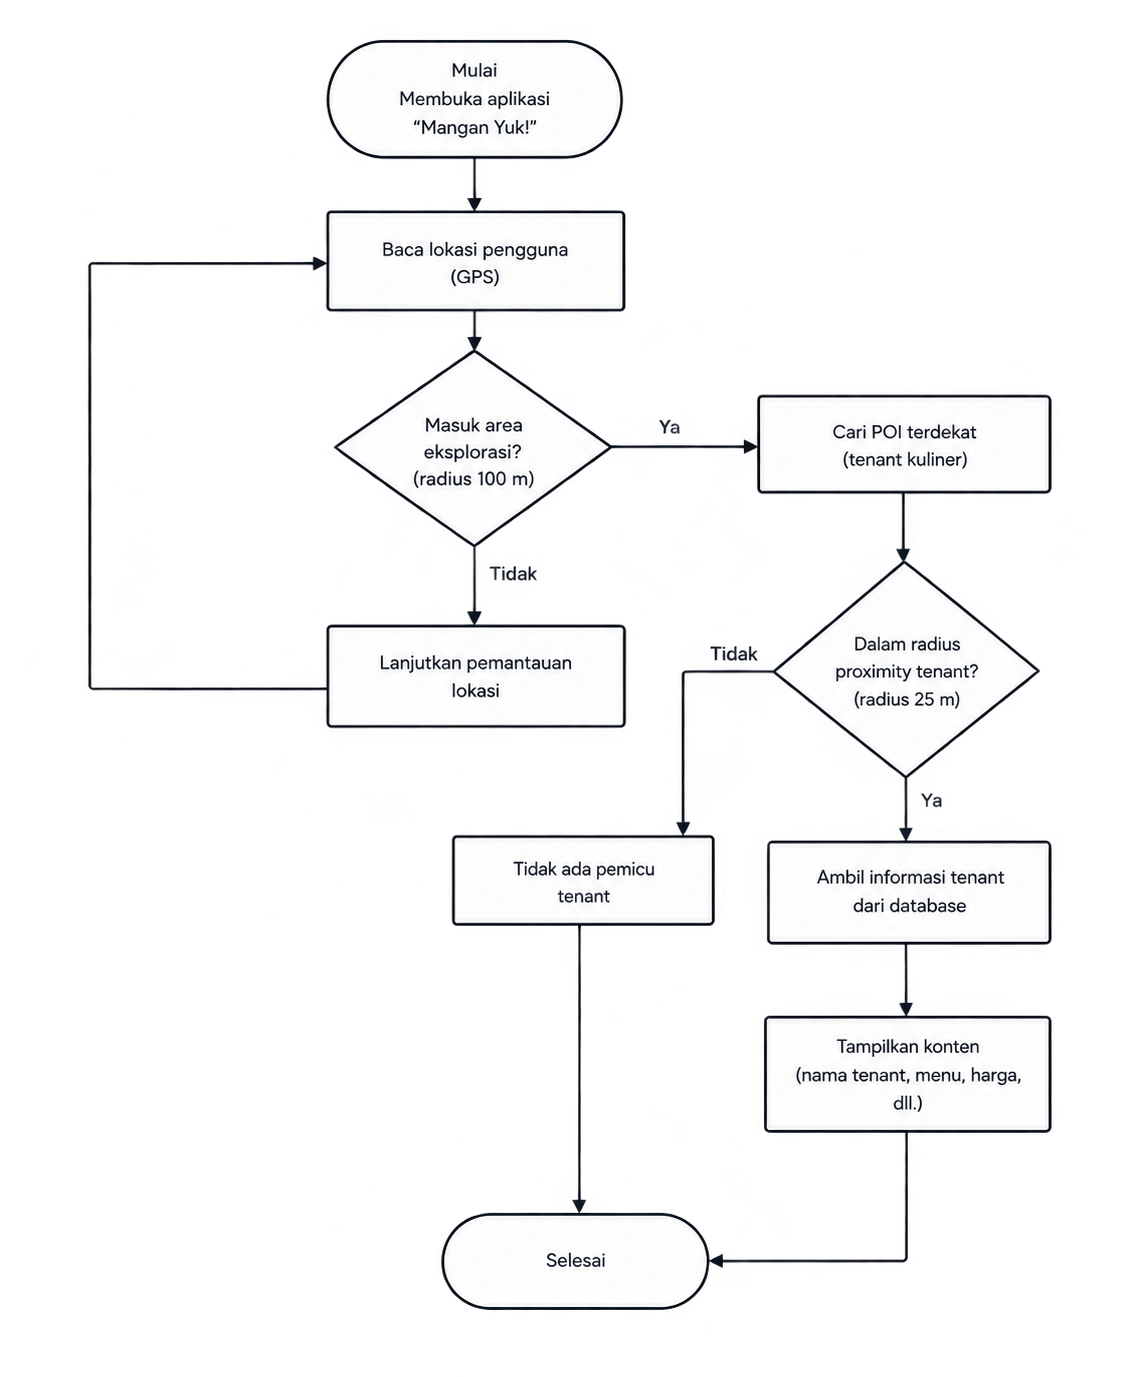
\includegraphics[width=0.6\textwidth,height=0.8\textheight,keepaspectratio]{images/diagram-location-trigger.png}
\caption{Diagram Location-Trigger Logic}
\label{fig:diagram-location-trigger}
\end{figure}

\subsection{Penjelasan Alur Logika}
\begin{enumerate}
  \item Pembacaan lokasi: aplikasi meminta izin lokasi kepada pengguna dan membaca koordinat GPS secara berkala ketika fitur eksplorasi aktif.
  \item Identifikasi POI: sistem mencari tenant yang berada dalam radius tertentu dari posisi pengguna.
  \item Pemeriksaan kondisi: sistem memeriksa apakah pengguna telah memasuki radius pemicu dan apakah informasi tenant tersebut sudah ditampilkan dalam sesi eksplorasi saat ini.
  \item Pemilihan konten: jika kondisi terpenuhi, sistem mengambil informasi tenant dari basis data. Informasi yang ditampilkan menggunakan data terstruktur dan aturan yang ditetapkan, bukan hasil generasi LLM.
  \item Respons sistem: aplikasi menampilkan kartu informasi atau pop-up. Pengguna dapat melihat detail tenant, membandingkan pilihan, atau melanjutkan ke POI berikutnya.
\end{enumerate}

\subsection{Contoh Skenario}

Radius pemicu setiap tenant adalah 10 meter. Ketika pengguna mendekati tenant tersebut hingga masuk ke radius itu, aplikasi memeriksa status pemicu. Jika informasinya belum ditampilkan pada sesi eksplorasi, aplikasi menampilkan kartu berisi nama tenant, kategori makanan, menu, dan harga. Jika pengguna masih berada di radius yang sama, \textit{pop-up} tidak ditampilkan berulang kali.
